\section{Intro to (Tin)flex}

\subsection{Idea}

Split the density distribution into multiple intervals for which better approximation for the \textit{hat} and \textit{squeeze} function can be constructed. Sample from the intervals using \textit{composition} and then for the selected intervals sample a value $x$ using the \textit{rejection with inversion} method.
For example in \autoref{fig:tf_example_normal} the normal distribution is split into six intervals with different hat and squeeze functions. The efficiency of the sampling can iteratily be improved by splitting more intervals and thus yielding a better approximation to the density.

\begin{figure}
    \centering
    \begin{subfigure}[b]{0.49\textwidth}
        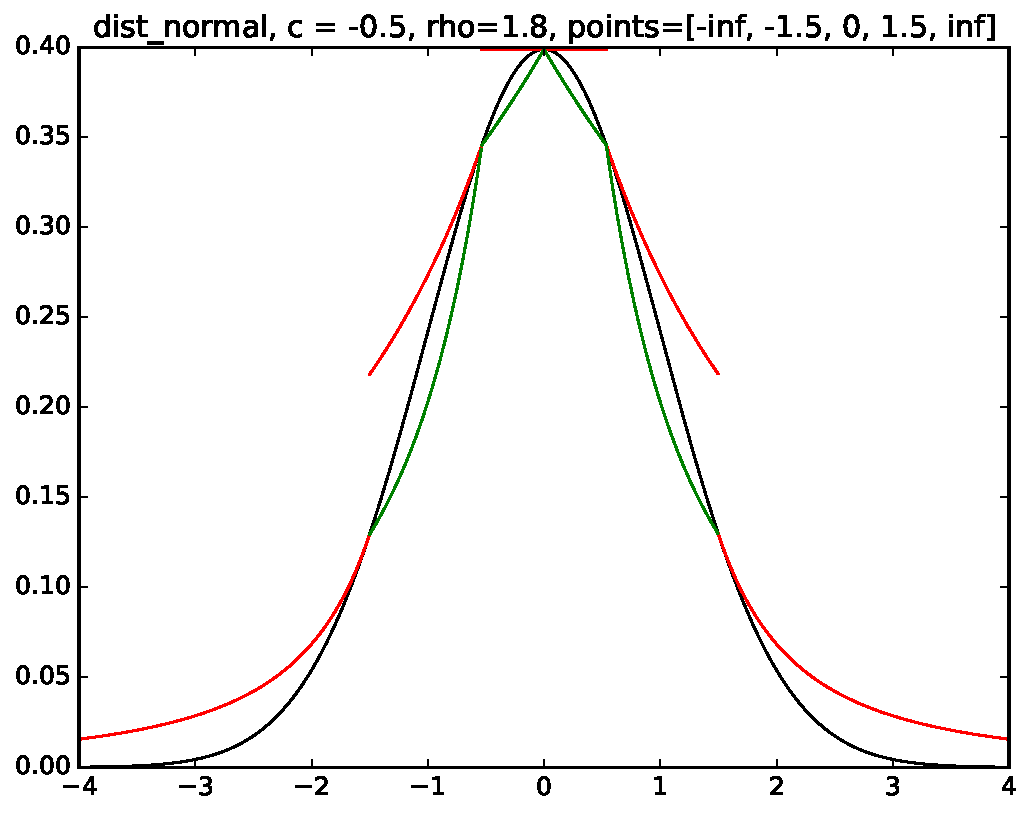
\includegraphics[width=\textwidth]{figs/tf_example_normal_6.pdf}
        \caption{$\rho = 1.8$, 6 intervals constructed}
    \end{subfigure}
    \begin{subfigure}[b]{0.49\textwidth}
        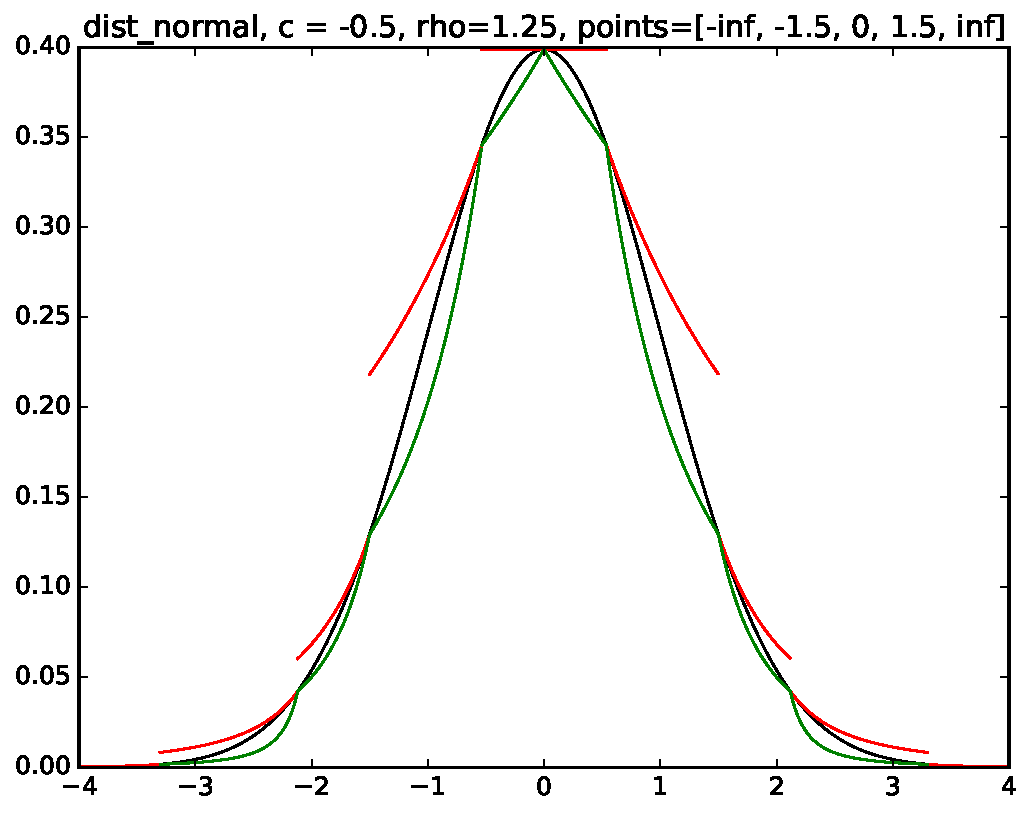
\includegraphics[width=\textwidth]{figs/tf_example_normal_10.pdf}
        \caption{$\rho = 1.25$, 10 intervals constructed}
    \end{subfigure}
    \centering
    \begin{subfigure}[b]{0.49\textwidth}
        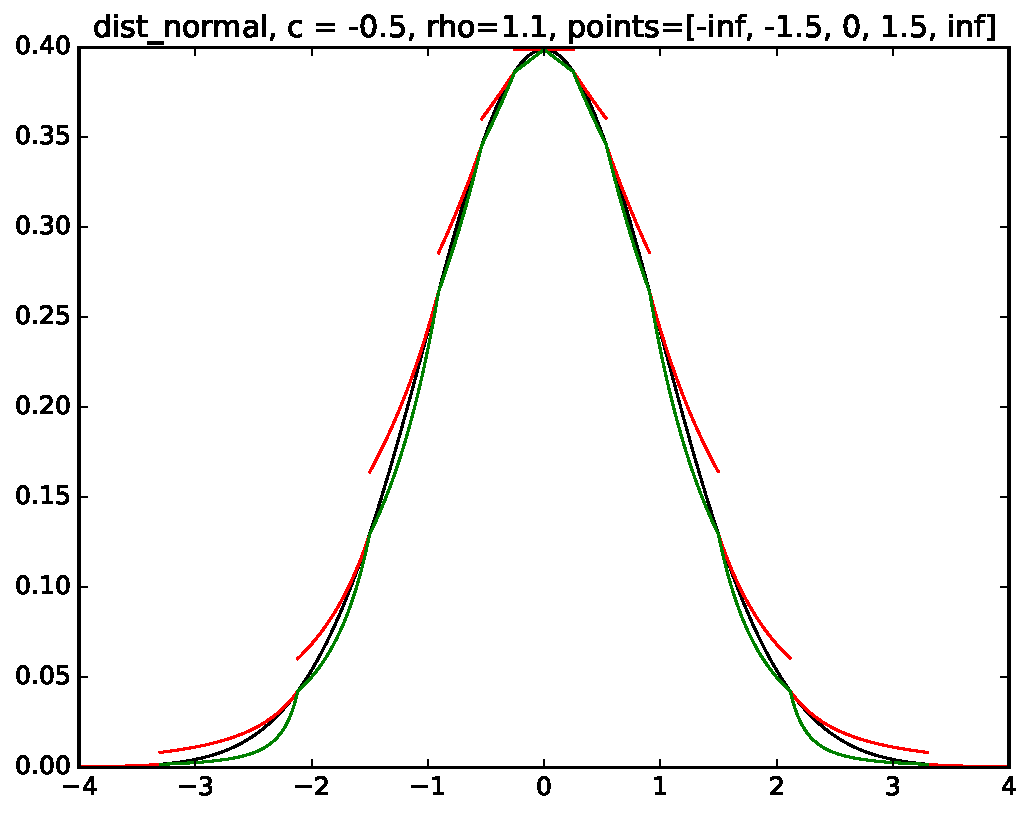
\includegraphics[width=\textwidth]{figs/tf_example_normal_14.pdf}
        \caption{$\rho = 1.1$, 14 intervals constructed}
    \end{subfigure}
    \begin{subfigure}[b]{0.49\textwidth}
        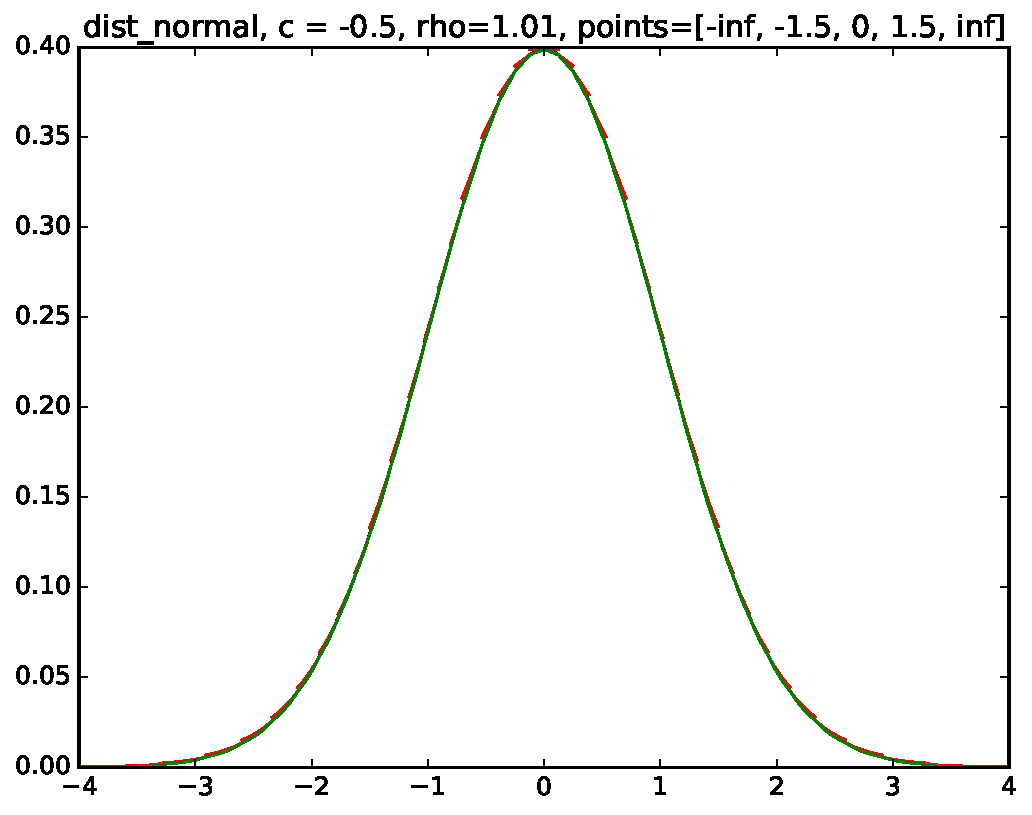
\includegraphics[width=\textwidth]{figs/tf_example_normal_44.pdf}
        \caption{$\rho = 1.01$, 44 intervals constructed}
    \end{subfigure}
    \caption{Flex algorithm for the normal distribution with different efficiencies $\rho$}
     \label{fig:tf_example_normal}
\end{figure}

\subsection{Transformations}

To approximate the hat and squeeze function Tinflex constructs linear functions when an interval is either concave or convex.
However as most distributions aren't \textit{concave}, but \textit{log-concave}, Tinflex uses a family of transformation of the pdf function as it operates in \textit{logspace} and can thus "force" most distributions to be concave. The transformations can be grouped in two classes:

\subsubsection{$c \neq 0$}

The general transformation function is $x^c$, however as inverse function is only defined in $\mathbb{C}$, we need to restrict it to positive numbers.

\[T_c(x) = sgn(c) * x^c\]

With the usual inversion rules we get if $c > 0$

\begin{align*}
y &= x^c \\
log(y) &= log(x^c) \\
log(y) &= c * log(x) \\
\frac{log(y)}{c} &= log(x) \\
exp\left(\frac{log(y)}{c}\right) &= x
\end{align*}

which is $y^{1 / c}$ and if $c < 0$:

\begin{align*}
y &= -x^c \\
log(y) &= log(-x^c) \\
log(y) &= -c * log(x) \\
\frac{log(y)}{c} &= -log(x) \\
exp\left(\frac{log(y)}{c}\right) &= -x
\end{align*}

which is $(-y)^{1 / c}$.
Thus in general we can define the inverse function as:

\[T_c^{-1}(x) = (sgn(c) * x)^{\frac{1}{c}}\]

An example of $T_c$ with $c = 2$ can be seen in \autoref{fig:sgn_pow} and for $c = -0.5$ in \autoref{fig:sgn_pow_0_5}.

Please note that (1) in the Tinflex paper and below this case is split into multiple common cases to have simpler formulas and reduce numerical errors. Furthermore (2) only with $c = 0$ the transformation is two-sided, thus for $c < 0$ $T^{-1}(x)$ is only defined for $x < 0$ in $\mathbb{R}$.

\begin{figure}[h!]
\centering
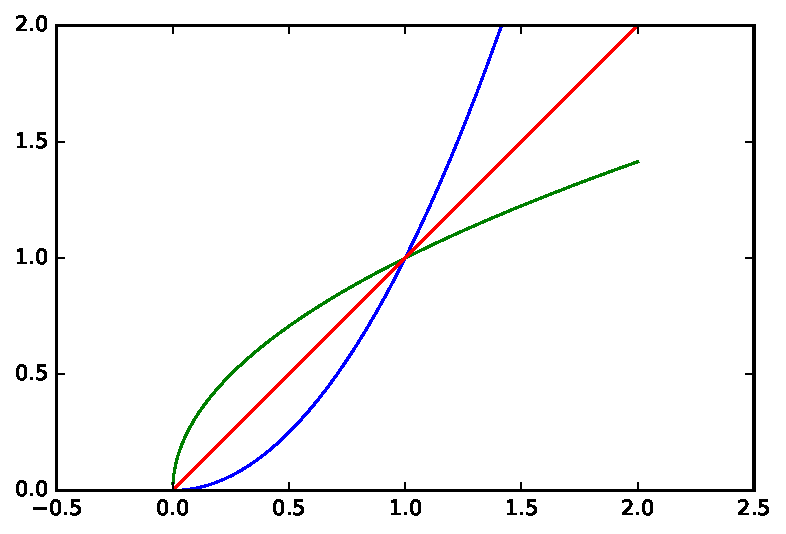
\includegraphics[width=0.8\textwidth]{figs/a_2_sgn_pow.pdf}
\caption{$x^2$ (red) and it's inverse $x^{1/2}$ (blue)}
\label{fig:sgn_pow}
\end{figure}

\begin{figure}[h!]
\centering
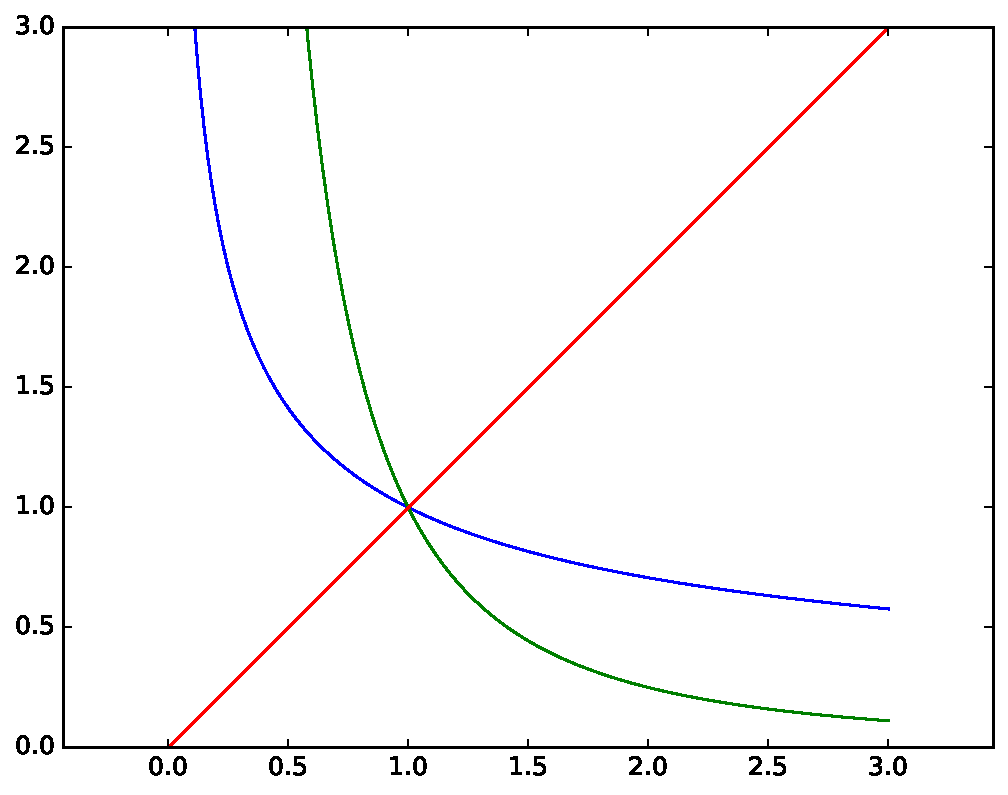
\includegraphics[width=0.8\textwidth]{figs/a_0_5_sgn_pow.pdf}
\caption{$-x^{-0.5}$ (red) and it's inverse $-x^{1/-0.5}$ (blue)}
\label{fig:sgn_pow_0_5}
\end{figure}

\pagebreak

\ \\

\pagebreak

\subsubsection{$c = 0$}

The special case for $c = 0$ needs to be made as division by zero isn't defined, however with this case the natural logarithm and exponential function is used.

\[T_c(x) = log(x)  \]

and it's inverse:

\[T_c^{-1}(x) = exp(x) \]

\begin{figure}[h]
\centering
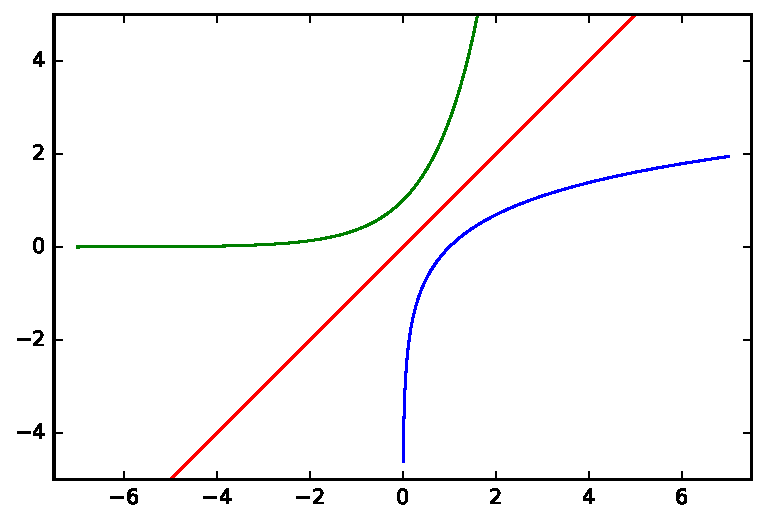
\includegraphics[width=0.8\textwidth]{figs/log_exp}
\caption{Exponential function (red) and it's inverse the natural log (blue)}
\label{fig:log_exp}
\end{figure}

\ \\

Moreover in accordance to the Tinflex paper $f(x)$ is the pdf, and $\tilde{f}(x)$ is its transformation.

\[\tilde{f}(x) = T_c(f(x))  \]

\subsubsection{Input of Tinflex}

Tinflex expects the \textbf{log}-density, which means that for $c = 0$, no transformations need to be applied.
However for $c \neq 0$ the inverse is needed, we first need to apply the \textit{inverse} $T_c^{-1}(x) = exp(x)$ and then apply the other $T_c$ transformation:

\begin{align*}
\tilde{f}(x) &= T_{c \neq 0}(T_0^{-1}(x))) \\
&= T_{c \neq 0}(exp(x))) \\
&= sgn(c) * exp(x)^c \\
&= sgn(c) * exp(x *c)
\end{align*}

\subsection{Linear functions}

The Tinflex paper uses the following definition for linear functions which are used in parts to construct hat and squeeze functions. The hat function majorizes the \textit{transformed} pdf, whereas the \textit{transformed} pdf majorizes the squeeze function.

\[ \tilde{f}(x) = \alpha + \beta * (x - x_0) \]

In the latter $h(x)$ will also be used instead of $\tilde{f}(x)$.
Remember that the transformation is applied with $T_c(x)$.

\subsection{Construction of linear functions}

For both secants and tangents $x_0$ and $\alpha$ within the interval $[\ell, r]$ are defined as follows:

\begin{enumerate}
\item $x_0$ is $\ell$ if $\tilde{f}(\ell) >= \tilde{f}(r)$, $r$ otherwise
\item $\alpha = \tilde{f}(x_0)$
\end{enumerate}

In fact only $\beta$ is defined differently: \\ 
\ \\
Tangent: $\beta = \tilde{f}'(x_0)$ \\ 
Secant:  $\beta = \frac{\tilde{f}(r) - \tilde{f}(\ell)}{r - \ell}$



